%!TEX root = ../main.tex
% \textit{[Lezione 13 (16-04-2020)]}
\chapter{Integrazione numerica}
Sia assegnata la funzione continua $f:[ a,b]\rightarrow \mathbb{R}$, supponiamo di volerne calcolare l'integrale definito
\begin{equation}
I(f) =\int\nolimits ^{b}_{a} f(x) \dx.
\label{eq:integrale}
\end{equation}
Calcolare analiticamente la primitiva di $f$ può essere complicato o addirittura impossibile.
L'idea è quindi quella di approssimare $f$ con un polinomio, con i metodi mostrati nel capitolo precedente, e calcolare l'integrale del polinomio approssimante:
\begin{equation*}
I(f) =\int\nolimits ^{b}_{a} f(x) \dx\approx I_{n}(f) =\int ^{b}_{a}\Pi _{n} f(x) \dx.
\end{equation*}
Se
$$\Pi _{n} f(x) =\sum\limits ^{n}_{i=0} f( x_{i})\mathcal{L}_{i}(x)$$
possiamo scrivere:
\begin{equation*}
I_{n}(f) =\underbrace{\int\limits ^{b}_{a}\sum\limits ^{n}_{i=0} f( x_{i})\mathcal{L}_{i}(x) \dx=\sum\limits ^{n}_{i=0} f( x_{i})\underbrace{\int\limits ^{b}_{a}\mathcal{L}_{i}(x) \dx.}_{\alpha _{i}}}_{\text{per linearità}}
\end{equation*}
Si noti che $\alpha _{i}$ non dipende dalla funzione che stiamo integrando, ma solo dall'intervallo di integrazione e dal $i$-esimo polinomio di Lagrange (cioè dal nodo $i$-esimo).
Quindi
\begin{equation}
I_{n}(f) =\sum\limits ^{n}_{i=0} \alpha _{i} \, f( x_{i})
\label{eq:formula-quadratura-interp}
\end{equation}
è una \textbf{formula di quadratura di tipo interpolatorio}\index{formula!di quadratura di tipo interpolatorio}.
\begin{itemize}
\item $x_{i} ,i=0,\dotsc ,n$ si chiamano \textbf{nodi di quadratura}\index{nodo!di quadratura};
\item $\alpha _{i} ,i=0,\dotsc ,n$ si chiamano \textbf{pesi di quadratura}\index{peso!di quadratura}.
\end{itemize}

Cerchiamo di quantificare l'errore compiuto approssimando l'integrale con l'interpolante: possiamo intuire che sia legato all'errore commesso nell'approssimazione del polinomio.
\section{Formule di quadratura semplici}
\subsection{Formula del punto medio}

Vediamo il caso $n=0$. Approssimiamo $f( x)$ come $\Pi _{0} f( x)$, cioè con il valore assunto nel punto medio dell'intervallo $[ a,b]$ detto $x_{0} =(a+b)/2$.
\begin{align*}
I( f) \approx I_{0}( f) & =\int\nolimits ^{b}_{a} \Pi _{0} f( x) \dx=\int\nolimits ^{b}_{a} f( x_{0})\mathcal{L}_{0}( x) \dx\\
 & =f( x_{0})\underbrace{\int\nolimits ^{b}_{a}\mathcal{L}_{0}( x) \dx}_{\alpha _{0}}\\
 & =f( x_{0}) \alpha _{0}.
\end{align*}
Il peso è quindi\footnote{Si noti che i polinomi di Lagrange saranno diversi tra i vari casi $n=0,1,2,\dotsc $ Per esempio nel caso $n=0$ è presente un solo nodo, quindi è sufficiente imporre che in $x_{0}$ valga $1$, ovvero è il polinomio costante $1$. Nel caso $n=1$ vi sono due nodi, quindi i polinomi dovranno rispettivamente valere $1$ in un nodo e $0$ nell'altro, avranno quindi espressioni diverse dal caso $n=0$.}
\begin{align*}
\alpha _{0} & =\int\nolimits ^{b}_{a}\mathcal{L}_{0}( x) \dx=\int\nolimits ^{b}_{a} \dx=[ x]^{b}_{a} =b-a,
\end{align*}
ovvero:
\begin{equation*}
I_{0}( f) =( b-a) f\left(\frac{a+b}{2}\right).
\end{equation*}

% Pattern Info

\begin{figure}[ht]
	\centering
	\tikzset{
	pattern size/.store in=\mcSize,
	pattern size = 5pt,
	pattern thickness/.store in=\mcThickness,
	pattern thickness = 0.3pt,
	pattern radius/.store in=\mcRadius,
	pattern radius = 1pt}
	\makeatletter
	\pgfutil@ifundefined{pgf@pattern@name@_ttl2ayssy}{
	\pgfdeclarepatternformonly[\mcThickness,\mcSize]{_ttl2ayssy}
	{\pgfqpoint{0pt}{-\mcThickness}}
	{\pgfpoint{\mcSize}{\mcSize}}
	{\pgfpoint{\mcSize}{\mcSize}}
	{
	\pgfsetcolor{\tikz@pattern@color}
	\pgfsetlinewidth{\mcThickness}
	\pgfpathmoveto{\pgfqpoint{0pt}{\mcSize}}
	\pgfpathlineto{\pgfpoint{\mcSize+\mcThickness}{-\mcThickness}}
	\pgfusepath{stroke}
	}}
	\makeatother
	\tikzset{every picture/.style={line width=0.75pt}} %set default line width to 0.75pt

	\begin{tikzpicture}[x=0.75pt,y=0.75pt,yscale=-1,xscale=1]
	%uncomment if require: \path (0,184); %set diagram left start at 0, and has height of 184

	%Shape: Axis 2D [id:dp6271010983380898]
	\draw  (163,138.38) -- (447.5,138.38)(182.5,28) -- (182.5,150.38) (440.5,133.38) -- (447.5,138.38) -- (440.5,143.38) (177.5,35) -- (182.5,28) -- (187.5,35)  ;
	%Shape: Rectangle [id:dp5635695594675718]
	\draw  [pattern=_ttl2ayssy,pattern size=6pt,pattern thickness=0.75pt,pattern radius=0pt, pattern color={rgb, 255:red, 155; green, 155; blue, 155}] (227.5,82.38) -- (359.5,82.38) -- (359.5,138.38) -- (227.5,138.38) -- cycle ;
	%Curve Lines [id:da6511035270825436]
	\draw [line width=1.5]    (227.5,92.38) .. controls (267.5,42.38) and (296.5,121.38) .. (359.5,63.38) ;

	% Text Node
	\draw (222,143.4) node [anchor=north west][inner sep=0.75pt]    {$a$};
	% Text Node
	\draw (354,143.4) node [anchor=north west][inner sep=0.75pt]    {$b$};
	% Text Node
	\draw (288,143.4) node [anchor=north west][inner sep=0.75pt]    {$x_{0}$};


	\end{tikzpicture}
	\caption{Formula del punto medio.}
\end{figure}

\subsection{Formula del trapezio}
Vediamo il caso $n=1$. Approssimiamo $f( x)$ come $\Pi _{1} f( x)$, cioè il polinomio di grado $1$ (una retta) che congiunge i due nodi (ovvero gli estremi), si ha
\begin{align*}
I( f) \approx I_{1}( f) & =\int\nolimits ^{b}_{a} \Pi _{1} f( x) \dx=\int\nolimits ^{b}_{a}\sum\limits ^{1}_{i=0} f( x_{i})\mathcal{L}_{i}( x) \dx\\
 & =f( a)\underbrace{\int\nolimits ^{b}_{a}\mathcal{L}_{0}( x) \dx}_{\alpha _{0}} +f( b)\underbrace{\int\nolimits ^{b}_{a}\mathcal{L}_{1}( x) \dx}_{\alpha _{1}}\\
 & =f( a) \alpha _{0} +f( b) \alpha _{1}.
\end{align*}
I pesi sono quindi
\begin{align*}
\alpha _{0} & =\int\nolimits ^{b}_{a}\mathcal{L}_{0}( x) \dx=\dotsc =\frac{b-a}{2}\\
\alpha _{1} & =\int\nolimits ^{b}_{a}\mathcal{L}_{1}( x) \dx=\dotsc =\frac{b-a}{2},
\end{align*}
ovvero:
\begin{equation*}
I_{1}( f) =( b-a)\left[\frac{f( a) +f( b)}{2}\right].
\end{equation*}

% Pattern Info

\begin{figure}[ht]
	\centering
	\tikzset{
	pattern size/.store in=\mcSize,
	pattern size = 5pt,
	pattern thickness/.store in=\mcThickness,
	pattern thickness = 0.3pt,
	pattern radius/.store in=\mcRadius,
	pattern radius = 1pt}
	\makeatletter
	\pgfutil@ifundefined{pgf@pattern@name@_d8nfo6cka}{
	\pgfdeclarepatternformonly[\mcThickness,\mcSize]{_d8nfo6cka}
	{\pgfqpoint{0pt}{-\mcThickness}}
	{\pgfpoint{\mcSize}{\mcSize}}
	{\pgfpoint{\mcSize}{\mcSize}}
	{
	\pgfsetcolor{\tikz@pattern@color}
	\pgfsetlinewidth{\mcThickness}
	\pgfpathmoveto{\pgfqpoint{0pt}{\mcSize}}
	\pgfpathlineto{\pgfpoint{\mcSize+\mcThickness}{-\mcThickness}}
	\pgfusepath{stroke}
	}}
	\makeatother
	\tikzset{every picture/.style={line width=0.75pt}} %set default line width to 0.75pt

	\begin{tikzpicture}[x=0.75pt,y=0.75pt,yscale=-1,xscale=1]
	%uncomment if require: \path (0,184); %set diagram left start at 0, and has height of 184

	%Shape: Polygon [id:ds914652478870901]
	\draw  [pattern=_d8nfo6cka,pattern size=6pt,pattern thickness=0.75pt,pattern radius=0pt, pattern color={rgb, 255:red, 155; green, 155; blue, 155}] (359.5,63.38) -- (359.5,138.38) -- (227.5,138.38) -- (227.5,92.38) -- cycle ;
	%Shape: Axis 2D [id:dp47963482701691174]
	\draw  (163,138.38) -- (447.5,138.38)(182.5,28) -- (182.5,150.38) (440.5,133.38) -- (447.5,138.38) -- (440.5,143.38) (177.5,35) -- (182.5,28) -- (187.5,35)  ;
	%Curve Lines [id:da17986572961517844]
	\draw [line width=1.5]    (227.5,92.38) .. controls (267.5,42.38) and (296.5,121.38) .. (359.5,63.38) ;

	% Text Node
	\draw (222,143.4) node [anchor=north west][inner sep=0.75pt]    {$a=x_{0}$};
	% Text Node
	\draw (354,143.4) node [anchor=north west][inner sep=0.75pt]    {$b=x_{1}$};
	\end{tikzpicture}
	\caption{Formula del trapezio.}
\end{figure}

\subsection{Formula di Cavalieri-Simpson}
Vediamo infine il caso $n=2$. Approssimiamo $f( x)$ come $\Pi _{2} f( x)$, cioè il polinomio di grado $2$ (una parabola) che congiunge i tre nodi, ovvero gli estremi e il punto medio dell'intervallo $[ a,b]$:
\begin{align*}
I( f) \approx I_{2}( f) & =\int\nolimits ^{b}_{a} \Pi _{2} f( x) \dx=\int\nolimits ^{b}_{a}\sum\limits ^{2}_{i=0} f( x_{i})\mathcal{L}_{i}( x) \dx\\
 & =f( a)\underbrace{\int\nolimits ^{b}_{a}\mathcal{L}_{0}( x) \dx}_{\alpha _{0}} +f\left(\frac{a+b}{2}\right)\underbrace{\int\nolimits ^{b}_{a}\mathcal{L}_{1}( x) \dx}_{\alpha _{1}} +f( b)\underbrace{\int\nolimits ^{b}_{a}\mathcal{L}_{2}( x) \dx}_{\alpha _{2}}\\
 & =f( a) \alpha _{0} +f\left(\frac{a+b}{2}\right) \alpha _{1} +f( b) \alpha _{2}.
\end{align*}
I pesi sono quindi
\begin{equation*}
\begin{aligned}
\alpha _{0} & =\int\nolimits ^{b}_{a}\mathcal{L}_{0}( x) \dx=\int\nolimits ^{b}_{a}\frac{( x-x_{1})( x-x_{2})}{( x_{0} -x_{1})( x_{0} -x_{2})} \dx=\dotsc =\frac{b-a}{6}\\
\alpha _{1} & =\int\nolimits ^{b}_{a}\mathcal{L}_{1}( x) \dx=\int\nolimits ^{b}_{a}\frac{( x-x_{2})( x-x_{0})}{( x_{1} -x_{0})( x_{1} -x_{2})} \dx=\dotsc =\frac{4}{6}( b-a)\\
\alpha _{2} & =\int\nolimits ^{b}_{a}\mathcal{L}_{2}( x) \dx=\int\nolimits ^{b}_{a}\frac{( x-x_{1})( x-x_{0})}{( x_{2} -x_{1})( x_{2} -x_{0})} \dx=\dotsc =\frac{b-a}{6},
\end{aligned}
\end{equation*}
ovvero:
\begin{equation*}
I_{2}( f) =\frac{b-a}{6}\left[ f( a) +4f\left(\frac{a+b}{2}\right) +f( b)\right].
\end{equation*}

% Pattern Info
\begin{figure}[ht]
	\centering
	\tikzset{
	pattern size/.store in=\mcSize,
	pattern size = 5pt,
	pattern thickness/.store in=\mcThickness,
	pattern thickness = 0.3pt,
	pattern radius/.store in=\mcRadius,
	pattern radius = 1pt}
	\makeatletter
	\pgfutil@ifundefined{pgf@pattern@name@_vam7h2eu6}{
	\pgfdeclarepatternformonly[\mcThickness,\mcSize]{_vam7h2eu6}
	{\pgfqpoint{0pt}{-\mcThickness}}
	{\pgfpoint{\mcSize}{\mcSize}}
	{\pgfpoint{\mcSize}{\mcSize}}
	{
	\pgfsetcolor{\tikz@pattern@color}
	\pgfsetlinewidth{\mcThickness}
	\pgfpathmoveto{\pgfqpoint{0pt}{\mcSize}}
	\pgfpathlineto{\pgfpoint{\mcSize+\mcThickness}{-\mcThickness}}
	\pgfusepath{stroke}
	}}
	\makeatother
	\tikzset{every picture/.style={line width=0.75pt}} %set default line width to 0.75pt

	\begin{tikzpicture}[x=0.75pt,y=0.75pt,yscale=-1,xscale=1]
	%uncomment if require: \path (0,184); %set diagram left start at 0, and has height of 184

	%Shape: Polygon Curved [id:ds0373113295724965]
	\draw  [pattern=_vam7h2eu6,pattern size=6pt,pattern thickness=0.75pt,pattern radius=0pt, pattern color={rgb, 255:red, 155; green, 155; blue, 155}] (227.5,99.38) .. controls (236.25,74.75) and (270.25,27.5) .. (292.75,22.75) .. controls (315.25,18) and (341.75,43.75) .. (359.5,70.38) .. controls (360.25,100.25) and (359.25,117.25) .. (359.5,145.38) .. controls (317.25,145.75) and (279.25,144.75) .. (227.5,145.38) .. controls (227.25,125.75) and (227.75,113.75) .. (227.5,99.38) -- cycle ;
	%Shape: Axis 2D [id:dp6749680858828806]
	\draw  (163,145.38) -- (447.5,145.38)(182.5,35) -- (182.5,157.38) (440.5,140.38) -- (447.5,145.38) -- (440.5,150.38) (177.5,42) -- (182.5,35) -- (187.5,42)  ;
	%Curve Lines [id:da5621088598250055]
	\draw [line width=1.5]    (227.5,99.38) .. controls (272.5,68.5) and (280.25,18.25) .. (307.25,17.25) .. controls (334.25,16.25) and (350.5,43.5) .. (359.5,70.38) ;
	%Straight Lines [id:da2688120029207004]
	\draw  [dash pattern={on 0.84pt off 2.51pt}]  (293.5,145.38) -- (293.5,22.75) ;

	% Text Node
	\draw (222,150.4) node [anchor=north west][inner sep=0.75pt]    {$a=x_{0}$};
	% Text Node
	\draw (354,150.4) node [anchor=north west][inner sep=0.75pt]    {$b=x_{1}$};
	\end{tikzpicture}
	\caption{Formula di Cavalieri-Simpson.}
\end{figure}

\section{Errore delle formule di quadratura semplici}
Studiamo l'accuratezza delle approssimazioni appena enunciate.
\begin{definition}
[Errore di quadratura]
\index{errore!di quadratura}
Siano
$$
  I(f) =\int ^{b}_{a} f(x) \dx
  \quad \text{e} \quad
  I_{n}(f) =\sum\limits ^{n}_{i=0} f( x_{i}) \alpha _{i}.
$$
Definiamo l'\textbf{errore di quadratura} come
\begin{equation*}
E_{n}(f) \coloneqq I(f) -I_{n}(f).
\end{equation*}
\end{definition}
\begin{definition}
[Grado di esattezza]
\index{grado!di esattezza}
Diciamo che una formula di quadratura ha \textbf{grado di esattezza} $r\geqslant 0$ se
\begin{equation*}
E_{n}( p_{r}) =0\quad \forall p_{r} \in \mathbb{P}^{r}.
\end{equation*}
\end{definition}
Enunciamo un utile criterio per determinare il grado di esattezza di una formula di quadratura.
\begin{theorem}
Una formula di quadratura ha grado di esattezza $r$ se e solo se 
\[E_n(x^k)=0\ \forall k=0,\dots,r\]
\end{theorem}

\subsection{Calcolo dell'errore}
Ricordiamo anzitutto il teorema della media integrale pesata.
\begin{theorem}
[Media integrale pesata]
\index{media integrale pesata}
Siano $f,g\in C^{0}([ a,b])$ tali che $g$ abbia segno costante in $( a,b)$.
Allora $\exists \xi \in [ a,b]$ tale che
\begin{equation*}
\int\nolimits ^{b}_{a} f(x) g(x) \dx=f( \xi )\int\nolimits ^{b}_{a} g(x) \dx.
\end{equation*}
\end{theorem}
Riportiamo ora i teoremi relativi agli errori delle tre formule presentate, dimostrando solo il primo\footnote{Le altre due dimostrazioni sono lasciate al lettore come esercizio.}.
\begin{theorem}
[Errore della formula del punto medio]
\index{errore!della formula del punto medio}
Data $f\in C^{2}([ a,b])$, esiste $\xi \in ( a,b)$ tale che
\begin{equation*}
E_{0}(f) =\frac{1}{24} f''( \xi )( b-a)^{3}.
\end{equation*}
\end{theorem}
\textit{Dimostrazione.}
Per ipotesi abbiamo:
\begin{equation*}
I(f) =\int\nolimits ^{b}_{a} f(x) \dx \quad \text e \quad I_{0}(f) =( b-a) f\underbrace{\left(\frac{a+b}{2}\right)}_{x_{m}}.
\end{equation*}
Supponiamo che $f$ sia sufficientemente regolare in modo da calcolare l'espansione di Taylor: $\exists \eta (x) \in ( x,x_{m})$ tale che
\begin{equation*}
f(x) =f( x_{m}) +( x-x_{m}) f'( x_{m}) +\frac{( x-x_{m})^{2}}{2} f''( \eta (x)).
\end{equation*}
Calcoliamo l'errore:
\begin{align*}
E_{0}(f) &= I(f) -\ I_{0}(f) \\
  &=\int\nolimits ^{b}_{a} f(x) \dx-( b-a) f( x_{m})\\
  &=\int\nolimits ^{b}_{a}[ f(x) -f( x_{m})] \dx\\
  &=\underbrace{\int\nolimits ^{b}_{a}( x-x_{m}) f'( x_{m}) \dx}_{A} +\underbrace{\int\nolimits ^{b}_{a}\frac{( x-x_{m})^{2}}{2} f''( \eta (x)) \dx}_{B}.
\end{align*}
\begin{itemize}
\item $A$ rappresenta l'integrale di una retta che passa per il punto medio dell'intervallo, quindi $A=f'( x_{m})\int\nolimits ^{b}_{a}( x-x_{m}) \dx=0$.
\item Per $B$ utilizziamo il teorema della media integrale pesata:
\end{itemize}
\begin{align*}
B & =\frac{1}{2}\int\nolimits ^{b}_{a}( x-x_{m})^{2} f''( \eta (x)) \dx\\
 & =\frac{1}{2} f''( \xi )\int\nolimits ^{b}_{a}( x-x_{m})^{2} \dx\\
 & =\frac{1}{6} f''( \xi )\left[( x-x_{m})^{3}\right]^{b}_{a}\\
 & =\frac{1}{24} f''( \xi )( b-a)^{3}.
\end{align*}
Allora otteniamo che:
\begin{gather*}
E_{0}(f) =A+B=\frac{1}{24} f''( \xi )( b-a)^{3}.
\qed
\end{gather*}
\begin{theorem}
[Errore della formula del trapezio]
\index{errore!della formula del trapezio}
Data $f\in C^{2}([ a,b])$, esiste $\xi _{2} \in ( a,b)$ tale che
\begin{equation*}
E_{1}(f) =-\frac{1}{12} f''( \xi _{2})( b-a)^{3}.
\end{equation*}
\end{theorem}
\begin{theorem}
[Errore della formula di Cavalieri-Simpson]
\index{errore!della formula di Cavalieri-Simpson}
Data $f\in C^{4}([ a,b])$, esiste $\xi _{3} \in ( a,b)$ tale che
\begin{equation*}
E_{2}(f) =-\frac{1}{90 \cdot 32} f^{(4)}( \xi _{3})( b-a)^{5}.
\end{equation*}
\end{theorem}
\textit{Osservazioni.}
\begin{enumerate}
\item Dall'espressione dell'errore di una formula di quadratura possiamo leggere il grado di esattezza:
\begin{enumerate}
\item nel caso $n=0$, ovvero l'errore della formula del punto medio, è presente la derivata seconda. Chiaramente in qualunque punto dell'intervallo, la derivata seconda di un polinomio di grado $1$ è sempre nulla, pertanto tutti i polinomi di grado fino a $1$ sono integrati esattamente da quella formula (cioè l'errore è nullo). Il grado di esattezza è quindi $1$.
\item nel caso $n=1$, ovvero l'errore della formula del trapezio, si ragiona analogamente e si deduce che il grado di esattezza è $1$, come nella formula del punto medio.
\item nel caso $n=2$, ovvero la formula di Cavalieri-Simpson, compare la derivata quarta. Il grado di esattezza è dunque $3$.
\end{enumerate}
\item Se $n$ è pari, il grado di esattezza è $n+1$, altrimenti è $n$.
\item Una formula di quadratura a $n+1$ nodi ha sempre grado di esattezza $\geqslant n$ perché $p_{n}(x) \equiv \Pi _{n} p_{n}(x)$, ovvero un polinomio coincide con il suo polinomio approssimante.
\item Le stime indicate hanno un'utilità limitata: includono il punto $\xi$ di cui è sconosciuta la posizione esatta. Per poterle utilizzare nella pratica, dobbiamo quindi passare alla norma infinito per limitare dall'alto l'errore:
\begin{equation*}
\begin{array}{ l }
| E_{0}(x)| \leqslant \frac{1}{24}( b-a)^{3}\underbrace{\Vert f''(x)\Vert _{\infty }}_{\leqslant C}\\
| E_{1}(x)| \leqslant \frac{1}{12}( b-a)^{3}\underbrace{\Vert f''(x)\Vert _{\infty }}_{\leqslant C}\\
| E_{2}(x)| \leqslant \frac{1}{90}\frac{1}{32}( b-a)^{5}\underbrace{\left\Vert f^{(4)}(x)\right\Vert _{\infty }}_{\leqslant C}.
\end{array}
\end{equation*}
\end{enumerate}

Torniamo al caso generale di una formula di tipo interpolatorio.
\begin{equation*}
\begin{drcases}
I(f) =\int\nolimits ^{b}_{a} f(x) \dx\\
I_{n}(f) =\int\nolimits ^{b}_{a} \Pi _{n} f(x) \dx
\end{drcases} \Rightarrow E_{n}(f) =\int\nolimits ^{b}_{a}\underbrace{[ f(x) -\Pi _{n} f(x)]}_{\text{errore del polinomio}} \dx.
\end{equation*}
\textit{Osservazione.} $E_{n}(f)$ erediterà tutti i problemi di stabilità dell'errore di interpolazione del polinomio su nodi equispaziati visti nella sezione \ref{sec:stabilita-pol-interpolazione}.
Aumentando $n$ per migliorare la qualità dell'approssimazione, ci scontriamo con il fenomeno di Runge nell'approssimazione del polinomio. Possiamo risolvere il problema usando:
\begin{itemize}
\item interpolazione composita, che darà origine alle formule di quadratura composite;
\item nodi non equispaziati, che daranno origine alle formule di quadratura su nodi non equispaziati.
\end{itemize}
\section{Formule di quadratura composite}

L'idea generale è molto semplice: dividiamo l'intervallo $[a,b]$ in $N$ sottointervalli di ampiezza $H$ ed applichiamo quanto visto a ciascun sottointervallo. Già dal primo caso sarà chiaro come l'uso di formule composite permette di raggiungere risultati migliori senza che sia necessario aumentare $n$, ottenendo formule parecchio complicate, ma semplicemente raffinando la griglia di sottointervalli (diminuendo $H$).

\subsection{Punto medio composito}
\index{metodo!del punto medio composito}
Fissiamo $N\geqslant 1$ e $H=(b-a)/N$. Ogni nodo è $x_{k} =a+kH$ con $k=0,1,\dotsc ,N$.
\begin{align*}
	I(f) =\int\nolimits ^{b}_{a} f(x) \dx & =\sum\limits ^{N-1}_{k=0}\underbrace{\int\nolimits ^{x_{k+1}}_{x_{k}} f(x) \dx}_{\text{formula del punto medio}} \\
	& \approx \sum\limits ^{N-1}_{k=0} Hf\left(\frac{x_{k} +x_{k+1}}{2}\right) =I^{c}_{0}(f).
\end{align*}

% Pattern Info
\begin{figure}[ht]
	\centering
	\tikzset{
	pattern size/.store in=\mcSize,
	pattern size = 5pt,
	pattern thickness/.store in=\mcThickness,
	pattern thickness = 0.3pt,
	pattern radius/.store in=\mcRadius,
	pattern radius = 1pt}
	\makeatletter
	\pgfutil@ifundefined{pgf@pattern@name@_eb0el2vf8}{
	\pgfdeclarepatternformonly[\mcThickness,\mcSize]{_eb0el2vf8}
	{\pgfqpoint{0pt}{-\mcThickness}}
	{\pgfpoint{\mcSize}{\mcSize}}
	{\pgfpoint{\mcSize}{\mcSize}}
	{
	\pgfsetcolor{\tikz@pattern@color}
	\pgfsetlinewidth{\mcThickness}
	\pgfpathmoveto{\pgfqpoint{0pt}{\mcSize}}
	\pgfpathlineto{\pgfpoint{\mcSize+\mcThickness}{-\mcThickness}}
	\pgfusepath{stroke}
	}}
	\makeatother

	% Pattern Info

	\tikzset{
	pattern size/.store in=\mcSize,
	pattern size = 5pt,
	pattern thickness/.store in=\mcThickness,
	pattern thickness = 0.3pt,
	pattern radius/.store in=\mcRadius,
	pattern radius = 1pt}
	\makeatletter
	\pgfutil@ifundefined{pgf@pattern@name@_b6h43mq3a}{
	\pgfdeclarepatternformonly[\mcThickness,\mcSize]{_b6h43mq3a}
	{\pgfqpoint{0pt}{-\mcThickness}}
	{\pgfpoint{\mcSize}{\mcSize}}
	{\pgfpoint{\mcSize}{\mcSize}}
	{
	\pgfsetcolor{\tikz@pattern@color}
	\pgfsetlinewidth{\mcThickness}
	\pgfpathmoveto{\pgfqpoint{0pt}{\mcSize}}
	\pgfpathlineto{\pgfpoint{\mcSize+\mcThickness}{-\mcThickness}}
	\pgfusepath{stroke}
	}}
	\makeatother

	% Pattern Info

	\tikzset{
	pattern size/.store in=\mcSize,
	pattern size = 5pt,
	pattern thickness/.store in=\mcThickness,
	pattern thickness = 0.3pt,
	pattern radius/.store in=\mcRadius,
	pattern radius = 1pt}
	\makeatletter
	\pgfutil@ifundefined{pgf@pattern@name@_wmkhgalp5}{
	\pgfdeclarepatternformonly[\mcThickness,\mcSize]{_wmkhgalp5}
	{\pgfqpoint{0pt}{-\mcThickness}}
	{\pgfpoint{\mcSize}{\mcSize}}
	{\pgfpoint{\mcSize}{\mcSize}}
	{
	\pgfsetcolor{\tikz@pattern@color}
	\pgfsetlinewidth{\mcThickness}
	\pgfpathmoveto{\pgfqpoint{0pt}{\mcSize}}
	\pgfpathlineto{\pgfpoint{\mcSize+\mcThickness}{-\mcThickness}}
	\pgfusepath{stroke}
	}}
	\makeatother

	% Pattern Info

	\tikzset{
	pattern size/.store in=\mcSize,
	pattern size = 5pt,
	pattern thickness/.store in=\mcThickness,
	pattern thickness = 0.3pt,
	pattern radius/.store in=\mcRadius,
	pattern radius = 1pt}
	\makeatletter
	\pgfutil@ifundefined{pgf@pattern@name@_os5131itn}{
	\pgfdeclarepatternformonly[\mcThickness,\mcSize]{_os5131itn}
	{\pgfqpoint{0pt}{-\mcThickness}}
	{\pgfpoint{\mcSize}{\mcSize}}
	{\pgfpoint{\mcSize}{\mcSize}}
	{
	\pgfsetcolor{\tikz@pattern@color}
	\pgfsetlinewidth{\mcThickness}
	\pgfpathmoveto{\pgfqpoint{0pt}{\mcSize}}
	\pgfpathlineto{\pgfpoint{\mcSize+\mcThickness}{-\mcThickness}}
	\pgfusepath{stroke}
	}}
	\makeatother
	\tikzset{every picture/.style={line width=0.75pt}} %set default line width to 0.75pt

	\begin{tikzpicture}[x=0.75pt,y=0.75pt,yscale=-1,xscale=1]
	%uncomment if require: \path (0,231); %set diagram left start at 0, and has height of 231

	%Shape: Axis 2D [id:dp4759406840395697]
	\draw  (109.44,185.72) -- (509.06,185.72)(136.83,30.69) -- (136.83,202.58) (502.06,180.72) -- (509.06,185.72) -- (502.06,190.72) (131.83,37.69) -- (136.83,30.69) -- (141.83,37.69)  ;
	%Shape: Rectangle [id:dp16625044527752886]
	\draw  [pattern=_eb0el2vf8,pattern size=6pt,pattern thickness=0.75pt,pattern radius=0pt, pattern color={rgb, 255:red, 155; green, 155; blue, 155}] (200.04,105.91) -- (246.5,105.91) -- (246.5,185.91) -- (200.04,185.91) -- cycle ;
	%Shape: Rectangle [id:dp15579631963983576]
	\draw  [pattern=_b6h43mq3a,pattern size=6pt,pattern thickness=0.75pt,pattern radius=0pt, pattern color={rgb, 255:red, 155; green, 155; blue, 155}] (246.5,101.91) -- (292.96,101.91) -- (292.96,185.91) -- (246.5,185.91) -- cycle ;
	%Shape: Rectangle [id:dp40434679147664454]
	\draw  [pattern=_wmkhgalp5,pattern size=6pt,pattern thickness=0.75pt,pattern radius=0pt, pattern color={rgb, 255:red, 155; green, 155; blue, 155}] (292.96,109.91) -- (339.42,109.91) -- (339.42,185.91) -- (292.96,185.91) -- cycle ;
	%Shape: Rectangle [id:dp9132938977615221]
	\draw  [pattern=_os5131itn,pattern size=6pt,pattern thickness=0.75pt,pattern radius=0pt, pattern color={rgb, 255:red, 155; green, 155; blue, 155}] (339.42,93.91) -- (385.88,93.91) -- (385.88,185.91) -- (339.42,185.91) -- cycle ;
	%Curve Lines [id:da974217190813893]
	\draw [line width=1.5]    (200.04,121.11) .. controls (256.23,50.88) and (296.96,161.84) .. (385.45,80.38) ;

	% Text Node
	\draw (157.89,196.26) node [anchor=north west][inner sep=0.75pt]    {$a=x_{0}$};
	% Text Node
	\draw (382.84,197.26) node [anchor=north west][inner sep=0.75pt]    {$b=x_{N}$};
	% Text Node
	\draw (237.89,196.26) node [anchor=north west][inner sep=0.75pt]    {$x_{1}$};
	% Text Node
	\draw (287.89,196.26) node [anchor=north west][inner sep=0.75pt]    {$x_{2}$};
	% Text Node
	\draw (260.89,189.26) node [anchor=north west][inner sep=0.75pt]    {$H$};
	\end{tikzpicture}
	\caption{Punto medio composito su $N$ intervalli di ampiezza $H$.}
\end{figure}

\begin{theorem}
Data $f\in C^{2}([ a,b])$, esiste $\xi \in ( a,b)$ tale che:
\begin{equation*}
E^{c}_{0}(f) =I(f) -I^{c}_{0}(f) =\frac{b-a}{24} H^{2} f''( \xi ).
\end{equation*}
Questo ha ordine di accuratezza 2 e grado di esattezza 1.
\end{theorem}
\begin{definition}
  \index{ordine!di accuratezza}
  L'esponente di $H$ è detto \textbf{ordine di accuratezza} della formula di quadratura. Dice quanto velocemente l'errore va a $0$ al tendere di $H$ a $0$, dove $H$ è l'ampiezza dell'intervallo.
\end{definition}

\subsection{Trapezio composito}
\index{metodo!del trapezio composito}
Fissiamo $N\geqslant 1$ e $H=(b-a)/N$. Ogni nodo è $x_{k} =a+kH$ con $k=0,1,\dotsc ,N$.
\begin{align*}
I(f) =\int\nolimits ^{b}_{a} f(x) \dx & =\sum\limits ^{N-1}_{k=0}\underbrace{\int\nolimits ^{x_{k+1}}_{x_{k}} f(x) \dx}_{\text{formula del trapezio}}\\
 & \approx \sum\limits ^{N-1}_{k=0}\frac{H}{2}[ f( x_{k}) +f( x_{k+1})] =I^{c}_{1}(f).
\end{align*}


% Pattern Info

\begin{figure}[ht]
	\centering
	\tikzset{
	pattern size/.store in=\mcSize,
	pattern size = 5pt,
	pattern thickness/.store in=\mcThickness,
	pattern thickness = 0.3pt,
	pattern radius/.store in=\mcRadius,
	pattern radius = 1pt}
	\makeatletter
	\pgfutil@ifundefined{pgf@pattern@name@_g0pxuakaj}{
	\pgfdeclarepatternformonly[\mcThickness,\mcSize]{_g0pxuakaj}
	{\pgfqpoint{0pt}{-\mcThickness}}
	{\pgfpoint{\mcSize}{\mcSize}}
	{\pgfpoint{\mcSize}{\mcSize}}
	{
	\pgfsetcolor{\tikz@pattern@color}
	\pgfsetlinewidth{\mcThickness}
	\pgfpathmoveto{\pgfqpoint{0pt}{\mcSize}}
	\pgfpathlineto{\pgfpoint{\mcSize+\mcThickness}{-\mcThickness}}
	\pgfusepath{stroke}
	}}
	\makeatother
	\tikzset{every picture/.style={line width=0.75pt}} %set default line width to 0.75pt

	\begin{tikzpicture}[x=0.75pt,y=0.75pt,yscale=-1,xscale=1]
	%uncomment if require: \path (0,240); %set diagram left start at 0, and has height of 240

	%Shape: Polygon [id:ds5086256767805182]
	\draw  [pattern=_g0pxuakaj,pattern size=6pt,pattern thickness=0.75pt,pattern radius=0pt, pattern color={rgb, 255:red, 155; green, 155; blue, 155}] (385.45,80.38) -- (385.45,185.72) -- (200.04,185.72) -- (200.04,121.11) -- (247.5,96.31) -- (292.75,108.72) -- (341.5,108.31) -- cycle ;
	%Shape: Axis 2D [id:dp9717194343072217]
	\draw  (109.44,185.72) -- (509.06,185.72)(136.83,30.69) -- (136.83,202.58) (502.06,180.72) -- (509.06,185.72) -- (502.06,190.72) (131.83,37.69) -- (136.83,30.69) -- (141.83,37.69)  ;
	%Curve Lines [id:da10369460307327572]
	\draw [line width=1.5]    (200.04,121.11) .. controls (256.23,50.88) and (296.96,161.84) .. (385.45,80.38) ;
	%Straight Lines [id:da907087688566599]
	\draw    (200.04,185.72) -- (385.45,185.72) (247.04,181.72) -- (247.04,189.72)(294.04,181.72) -- (294.04,189.72)(341.04,181.72) -- (341.04,189.72) ;

	% Text Node
	\draw (157.89,196.26) node [anchor=north west][inner sep=0.75pt]    {$a=x_{0}$};
	% Text Node
	\draw (382.84,197.26) node [anchor=north west][inner sep=0.75pt]    {$b=x_{N}$};
	% Text Node
	\draw (237.89,196.26) node [anchor=north west][inner sep=0.75pt]    {$x_{1}$};
	% Text Node
	\draw (287.89,196.26) node [anchor=north west][inner sep=0.75pt]    {$x_{2}$};
	% Text Node
	\draw (260.89,189.26) node [anchor=north west][inner sep=0.75pt]    {$H$};


	\end{tikzpicture}
	\caption{Trapezio composito su $N$ intervalli di ampiezza $H$.}
\end{figure}

\begin{theorem}
Data $f\in C^{2}([ a,b])$, esiste $\eta \in ( a,b)$ tale che:
\begin{equation*}
E^{c}_{1}(f) =I(f) -I^{c}_{1}(f) =-\frac{b-a}{12} H^{2} f''( \eta ).
\end{equation*}
Questo ha ordine di accuratezza 2 e grado di esattezza 1.
\end{theorem}

\subsection{Cavalieri-Simpson composito}
\index{metodo!di Cavalieri-Simpson composito}
Fissiamo $N\geqslant 1$ e $H=\frac{b-a}{N}$. Ogni nodo è $x_{k} =a+kH$ con $k=0,1,\dotsc ,N$.
\begin{equation*}
\begin{aligned}
I(f) =\int\nolimits ^{b}_{a} f(x) \dx & =\sum\limits ^{N-1}_{k=0}\underbrace{\int\nolimits ^{x_{k+1}}_{x_{k}} f(x) \dx}_{\text{formula di CS}}\\
 & \approx \sum\limits ^{N-1}_{k=0}\frac{H}{6}\left[ f( x_{k}) +4f\left(\frac{x_{k} +x_{k+1}}{2}\right) +f( x_{k+1})\right] =I^{c}_{2}(f).
\end{aligned}
\end{equation*}
\begin{theorem}
Data $f\in C^{4}([ a,b])$, esiste $\zeta \in ( a,b)$ tale che:
\begin{equation*}
E^{c}_{2}(f) =I(f) -I^{c}_{2}(f) =-\frac{b-a}{180}\frac{1}{16} H^{4} f^{(4)}( \zeta ).
\end{equation*}
Questo ha ordine di accuratezza 4 e grado di esattezza 3.
\end{theorem}
% \textit{[Lezione 14 (20-04-2020)]}

\textit{Esempio.} Calcoliamo l'errore commesso usando la formula del punto medio su
\begin{gather*}
I(f) =\int\nolimits ^{\pi }_{0} f(x) \dx \quad \text{con} \quad f(x) =\sin(x).
\end{gather*}
Abbiamo dunque che:
\begin{gather*}
\begin{aligned}
E_{0}(f) & =\frac{1}{24}( b-a)^{3} f''( \xi ) \quad \xi \in [ a,b]\\
 & =\frac{1}{24}( \pi -0)^{3} f''( \xi )\\
| E_{0}(f)|  & \leqslant \frac{\pi ^{3}}{24}\Vert f''(x)\Vert _{\infty }=\frac{\pi ^{3} }{24} \max_{x\in [ 0,\pi ]}| -\sin x| \leqslant \frac{\pi ^{3}}{24}.
\end{aligned}
\end{gather*}

\section{Formule di Newton-Cotes (NC)}
\index{formula!di Newton-Cotes}
Sono basate sul metodo di interpolazione di Lagrange su nodi \textit{equispaziati}, nonché una generalizzazione dei metodi visti finora.
Fissiamo $n >0$ e indichiamo i nodi di quadratura con:
\begin{equation*}
x_{k} =x_{0} +kh \quad \text{con} \quad k=0,\dotsc ,n\quad \text{dove} \quad h=\frac{b-a}{n}.
\end{equation*}
% un bel nitpick: la n è diventata N? Vogliamo uniformare la notazione? (AW)
La formula generale è data da:
\begin{equation*}
I_{n}(f) =\sum\limits ^{n}_{i=0} \alpha _{i} f( x_{i}).
\end{equation*}
Le formule del punto medio, del trapezio e la formula di Simpson sono esempi di formule di Newton-Cotes, dove, rispettivamente, $n=0$, $n=1$ e $n=2$. Nel caso generale si definiscono:
\begin{itemize}
\item \textbf{formule aperte}\index{formula!aperta}, quelle in cui $x_{0} =a+h,x_{n} =b-h,h=(b-a)/(n+2)$ con $n\geqslant 0$, per esempio le formule di punto medio;
\item \textbf{formule chiuse}\index{formula!chiusa}, quelle in cui $x_{0} =a,x_{n} =b,h=(b-a)(n)$ con $n \geqslant 1$, per esempio le formule del trapezio e di Cavalieri-Simpson.
\end{itemize}

\textbf{Proprietà.}
Le formule di Newton-Cotes hanno pesi di quadratura $\alpha _{i}$ che dipendono solo da $n$ e da $h$, ma non dall’intervallo di integrazione $[ a,b]$.

\textit{Dimostrazione.}
Per semplicità consideriamo il caso delle formule di NC chiuse. Effettuiamo il seguente cambio di variabile:
\begin{equation*}
x=\Psi (t) =x_{0} +th\quad ( = a+th)
\end{equation*}
e notiamo che:
\begin{equation*}
\Psi (0) =a\qquad \Psi (n) =b\qquad \Psi (k) =x_{k} \quad \text{con} \quad k=0,\dotsc ,n.
\end{equation*}
Si vogliono ora calcolare le frazioni dei polinomi di Lagrange:
\begin{equation*}
\frac{x-x_{k}}{x_{i} -x_{k}} =\frac{a+th-( a+kh)}{a+ih-( a+kh)} =\frac{h( t-k)}{h( i-k)} =\frac{t-k}{i-k},
\end{equation*}
ma quindi
\begin{equation*}
\mathcal{L}_{i} (x)=\prod ^{n}_{k=0,k\neq i}\frac{x-x_{k}}{x_{i} -x_{k}} =\prod ^{n}_{k=0,k\neq i}\frac{t-k}{i-k} :=\varphi _{i}(t) \qquad \text{con } 0\leqslant i\leqslant n.
\end{equation*}
Usando l'uguaglianza $\alpha _{i} =\int ^{b}_{a}\mathcal{L}_{i}(x) \dx$ otteniamo che
\begin{equation*}
\alpha _{i} =\int\nolimits ^{b}_{a}\mathcal{L}_{i}(x) \dx=\int\nolimits ^{n}_{0} \varphi _{i}(t) hdt=h\int\nolimits ^{n}_{0} \varphi _{i}(t) \dt
\end{equation*}
da cui si ottiene la formula di quadratura
\begin{equation*}
I_{n}(f) =h\sum\limits ^{n}_{i=0} w_{i} f( x_{i}) ,\quad w_{i} =\int\nolimits ^{n}_{0} \varphi _{i}(t) \dt.
\qed
\end{equation*}
\textit{Osservazione.} Si può svolgere un ragionamento analogo per le formule di NC aperte, ottenendo:
\begin{equation*}
I_{n}(f) =h\sum\limits ^{n}_{i=0} w_{i} f( x_{i}) ,\quad w_{i} =\int\nolimits ^{n+1}_{-1} \varphi _{i}(t) \dt.
\end{equation*}
Nelle seguenti tabelle sono visualizzati i pesi delle formule di quadratura di Newton-Cotes chiuse e aperte:

\begin{table}[H]
\centering
{\renewcommand{\arraystretch}{1.3}% for the vertical padding
\caption{Pesi delle formule di Newton-Cotes}
\begin{subtable}{.5\linewidth}
\centering
\caption{Chiuse}
\begin{tabular}{ccccccc}
\toprule
 $n$ & $1$ & $2$ & $3$ & $4$ & $5$ & $6$ \\
\midrule
 $w_{0}$ & $\frac{1}{2}$ & $\frac{1}{3}$ & $\frac{3}{8}$ & $\frac{14}{45}$ & $\frac{95}{288}$ & $\frac{41}{140}$ \\
$w_{1}$ & $0$ & $\frac{4}{3}$ & $\frac{9}{8}$ & $\frac{64}{45}$ & $\frac{375}{288}$ & $\frac{216}{140}$ \\
$w_{2}$ & $0$ & $0$ & $0$ & $\frac{24}{45}$ & $\frac{250}{288}$ & $\frac{27}{140}$ \\
$w_{3}$ & $0$ & $0$ & $0$ & $0$ & $0$ & $\frac{272}{140}$ \\
 \bottomrule
\end{tabular}
\end{subtable}%

\begin{subtable}{.5\linewidth}
\centering
\caption{Aperte}
\begin{tabular}{ccccccc}
\toprule
 $n$ & $0$ & $1$ & $2$ & $3$ & $4$ & $5$ \\
\midrule
 $w_{0}$ & 2 & $\frac{3}{2}$ & $\frac{8}{3}$ & $\frac{5}{24}$ & $\frac{66}{20}$ & $\frac{4277}{1440}$ \\
$w_{1}$ & $0$ & $0$ & $-\frac{4}{3}$ & $\frac{5}{24}$ & $-\frac{84}{20}$ & $-\frac{3171}{1440}$ \\
$w_{2}$ & $0$ & $0$ & $0$ & $0$ & $\frac{156}{20}$ & $\frac{3934}{1440}$ \\
 \bottomrule
\end{tabular}
\end{subtable}%

}
\end{table}

\begin{theorem}
[Errore delle formule di Newton-Cotes]
\index{errore!delle formule di Newton-Cotes}
Data una formula di Newton-Cotes con $n$ pari, aperta o chiusa, e data $f\in C^{n+2}([ a,b])$, l'errore è dato da:
\begin{equation}
E_{n}(f) =\frac{M_{n}}{( n+2) !} h^{n+3} f^{( n+2)}( \xi )
\label{eq:errore-newton-cotes}
\end{equation}
dove $\xi \in ( a,b)$ e
\begin{equation*}
M_{n} =\begin{cases}
\int^{n}_{0} t\ \pi _{n+1}(t) \dt< 0 & \text{per formule chiuse}\\
\int^{n+1}_{-1} t\ \pi _{n+1}(t) \dt >0 & \text{per formule aperte}
\end{cases}
\end{equation*}
e dove
$$\pi _{n+1}(t) =\prod\limits ^{n}_{i=0}( t-i).$$
Dalla \eqref{eq:errore-newton-cotes} si deduce che il grado di esattezza è pari a $n+1$ e che l'ordine di accuratezza è $h^{n+3}$.

Similmente, per $n$ dispari e $f\in C^{n+1}([ a,b])$, si ha
\begin{equation}
E_{n}(f) =\frac{K_{n}}{( n+1) !} h^{n+2} f^{( n+1)}( \eta ),
\label{eq:errore-newton-cotes2}
\end{equation}
con
\begin{equation*}
K_{n} =\begin{cases}
\int\nolimits ^{n}_{0} \pi _{n+1}(t) \dt< 0 & \text{per formule chiuse} \\
\int\nolimits ^{n+1}_{-1} \pi _{n+1}(t) \dt >0 & \text{per formule aperte}
\end{cases}
\end{equation*}
dunque il grado di esattezza è $n$ e l'ordine di accuratezza è $h^{n+2}$.
\end{theorem}
Si noti che i pesi delle formule di NC non hanno segno costante, e ciò può essere fonte di errore di cancellazione\footnote{L'errore di cancellazione avviene quando il calcolatore somma due numeri molto piccoli e di segno opposto, a causa del fatto che esso può rappresentare solo un numero \textit{finito} di cifre decimali. Per esempio valutando le due forme del polinomio $p( x) =( x-1)^{6} =x^{6} -6x^{5} +15x^{4} -20x^{3} +15x^{2} -6x+1$ su un intervallo molto fine si noteranno delle oscillazioni, anche se il polinomio è lo stesso.}.

Inoltre da $n=9$ in poi le costanti che entrano nella formula dell'errore tendono a diventare troppo grandi, motivo per cui cercheremo di guadagnare qualcosa in termini grado di esattezza e ordine di accuratezza con le formule composite e con l'integrazione su nodi non equispazioni (Integrazione Gaussiana) nelle sezioni \ref{sec:newton-cotes-composite} e \ref{sec:integrazione-gaussiana}.

\section{Formule di Newton-Cotes composite}
\label{sec:newton-cotes-composite}
\index{formula!di Newton-Cotes composite}
Dividiamo $[ a,b]$ in $m$ sottointervalli $T_{j} =[ y_{j} ,y_{j+1}]$, tali che $y_{i} =a+jH$, essendo $H=(b-a)/m$, per $j=0,\dotsc ,m$.

\begin{figure}[htpb]
	\centering
	\tikzset{every picture/.style={line width=0.75pt}} %set default line width to 0.75pt

	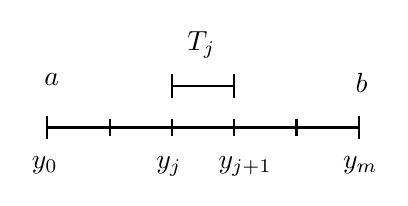
\begin{tikzpicture}[x=0.75pt,y=0.75pt,yscale=-1,xscale=1]
	%uncomment if require: \path (0,102); %set diagram left start at 0, and has height of 102

	%Straight Lines [id:da20621224248267156]
	\draw    (250,30) -- (280,30) ;
	\draw [shift={(280,30)}, rotate = 180] [color={rgb, 255:red, 0; green, 0; blue, 0 }  ][line width=0.75]    (0,5.59) -- (0,-5.59)   ;
	\draw [shift={(250,30)}, rotate = 180] [color={rgb, 255:red, 0; green, 0; blue, 0 }  ][line width=0.75]    (0,5.59) -- (0,-5.59)   ;
	%Straight Lines [id:da9554369535839922]
	\draw    (190,50) -- (340,50) (220,46) -- (220,54)(250,46) -- (250,54)(280,46) -- (280,54)(310,46) -- (310,54) ;
	\draw [shift={(340,50)}, rotate = 180] [color={rgb, 255:red, 0; green, 0; blue, 0 }  ][line width=0.75]    (0,5.59) -- (0,-5.59)   ;
	\draw [shift={(190,50)}, rotate = 180] [color={rgb, 255:red, 0; green, 0; blue, 0 }  ][line width=0.75]    (0,5.59) -- (0,-5.59)   ;

	% Text Node
	\draw (187,22.4) node [anchor=north west][inner sep=0.75pt]    {$a$};
	% Text Node
	\draw (337,22.4) node [anchor=north west][inner sep=0.75pt]    {$b$};
	% Text Node
	\draw (181,62.4) node [anchor=north west][inner sep=0.75pt]    {$y_{0}$};
	% Text Node
	\draw (241,62.4) node [anchor=north west][inner sep=0.75pt]    {$y_{j}$};
	% Text Node
	\draw (271,62.4) node [anchor=north west][inner sep=0.75pt]    {$y_{j+1}$};
	% Text Node
	\draw (256,2.4) node [anchor=north west][inner sep=0.75pt]    {$T_{j}$};
	% Text Node
	\draw (331,62.4) node [anchor=north west][inner sep=0.75pt]    {$y_{m}$};


	\end{tikzpicture}
\end{figure}
\FloatBarrier

Si utilizza quindi in ogni sottointervallo una formula interpolatoria avente per nodi i punti $\left\{x^{(j)}_{k} ,\ 0\leqslant k\leqslant n\right\}$ e per pesi i coefficienti $\left\{\alpha ^{(j)}_{k} ,\ 0\leqslant k\leqslant n\right\}$. Poiché
\begin{equation*}
I(f) =\int ^{b}_{a} f(x) \dx=\sum\limits ^{m-1}_{j=0}\int\nolimits _{T_{j}} f(x) \dx=\sum\limits ^{m-1}_{j=0}\int\nolimits ^{y_{j+} 1}_{y_{j}} f(x) \dx,
\end{equation*}
si può ottenere una formula di quadratura interpolatoria composita sostituendo $I(f)$ con
\begin{equation*}
I_{n,m}(f) =\sum\limits ^{m-1}_{j=0}\sum\limits ^{n}_{k=0} \alpha ^{(j)}_{k} f\left( x^{(j)}_{k}\right).
\end{equation*}
\begin{theorem}
[Errore delle formule di Newton-Cotes composite]
\index{errore!delle formule di Newton-Cotes composite}
Data una formula di Newton-Cotes composita, aperta o chiusa su ogni sottointervallo e con $n$ pari, se $f\in C^{n+2}([ a,b])$, si ha, per $\xi \in ( a,b)$:
\begin{equation*}
E_{n,m}(f) =\frac{b-a}{( n+2) !}\frac{M_{n}}{\gamma ^{n+3}_{n}} H^{n+2} f^{( n+2)}( \xi ).
\end{equation*}
Nel caso in cui $n$ sia dispari, se $f\in C^{n+1}([ a,b])$, si ha invece, per $\eta \in ( a,b)$:
\begin{equation*}
E_{n,m}(f) =\frac{b-a}{( n+1) !}\frac{K_{n}}{\gamma ^{n+2}_{n}} H^{n+1} f^{( n+1)}( \eta ).
\end{equation*}

Nelle due formule è stato definito
\begin{equation*}
\gamma _{n} =\begin{cases}
n+2 & \text{per formule aperte}\\
n & \text{per formule chiuse}.
\end{cases}
\end{equation*}
\end{theorem}

% \textit{[Lezione 15 (21-04-2020)]}
\section{Quadratura su nodi non equispaziati (Integrazione Gaussiana)}
\label{sec:integrazione-gaussiana}

Possiamo guadagnare gradi di esattezza e ordini di accuratezza usando nodi non equispaziati con le \textbf{formule di quadratura di Gauss-Legendre}\index{formula!di Gauss-Legendre} (GL) o di \textbf{Gauss-Legendre-Lobatto}\index{formula!di Gauss-Legendre-Lobatto} (GLL).

I nodi e i pesi sono scelti in modo da massimizzare il grado di esattezza.

In particolare:
\begin{equation*}
\{( x_{i} ,\alpha _{i})\}^{n}_{i=0} \ \ \rightarrow \ \ I_{n}(f) =\sum\limits ^{n}_{i=0} \alpha _{i} f( x_{i}) \ \begin{cases}
\text{g.d.e.} =( 2n+1) & \text{con GL}\\
\text{g.d.e.} =( 2n-1) & \text{con GLL.}
\end{cases}
\end{equation*}

\subsection{Nodi e pesi di Gauss-Legendre (GL)}
Poiché abbiamo $n+1$ nodi e $n+1$ pesi, bisogna imporre $2n+2$ condizioni per determinarli. Imponiamo che la formula di quadratura esattamente tutti i polinomi fino al grado $2n+1$, cioè:
\[
\begin{cases}
    \text{g.d.e.}=0\\
    \text{g.d.e.}=1\\
    \vdots\\
    \text{g.d.e.}=2n+1
\end{cases}
\]
Queste sono $2n+2$ equazioni, che permettono di determinare i \textbf{nodi di Gauss-Legendre}\index{nodi!di Gauss-Legendre} e i relativi pesi.

\textit{Esempio.} Determiniamo nodi e pesi di GL per $n=1$.
\[
\begin{cases}
    \text{g.d.e.}=0\\
    \text{g.d.e.}=1\\
    \text{g.d.e.}=2\\
    \text{g.d.e.}=3
\end{cases}\iff 
\begin{cases}
    \int_a^b 1=b-a=\alpha_0+\alpha_1\\
    \int_a^b x=\frac{b^2}2-\frac{a^2}2=\alpha_0 x_0+\alpha_1 x_1\\
    \int_a^b x^2=\frac{b^3}3-\frac{a^3}3=\alpha_0 x_0^2+\alpha_1 x_1^2\\
    \int_a^b x^3=\frac{b^4}4-\frac{a^4}4=\alpha_0 x_0^3+\alpha_1 x_1^3
\end{cases}
\]
È un sistema non lineare, difficile da risolvere. La sua soluzione è 
\[
x_1= a+\left(1-\frac1{\sqrt 3}\right)\left(\frac{b-a}2\right),\quad x_2= a+\left(1+\frac1{\sqrt 3}\right)\left(\frac{b-a}2\right),\quad \alpha_1=\alpha_2 =\frac{b-a}{2}
\]
\textit{Osservazione.} La formula di quadratura di GL è quindi una formula aperta.

\begin{theorem}
    [Errore della formula di Gauss-Legendre a 2 nodi]
    Data $f\in C^4([a,b])$, esiste $\xi_\text{G2}\in[a,b]$ tale che 
    \[
    E_\text{G2}(f)=\frac{1}{4320} (b-a)^5f^{(4)}(\xi_\text{G2})
    \]
\end{theorem}
Quindi con due nodi abbiamo prestazioni paragonabili a Cavalieri-Simpson!

\textit{Esempio.}
Integriamo su $( -1,1)$, con $n=1$. Abbiamo $2$ nodi, i cui pesi, si può verificare, sono $\alpha _{i} =\{1,1\}$ mentre i nodi sono $x_{i} =\left\{\pm 1/\sqrt{3}\right\}$. Consideriamo una $f( x) ,x\in [ -1,1]$.

\begin{figure}[ht]
	\centering
	\tikzset{every picture/.style={line width=0.75pt}} %set default line width to 0.75pt

	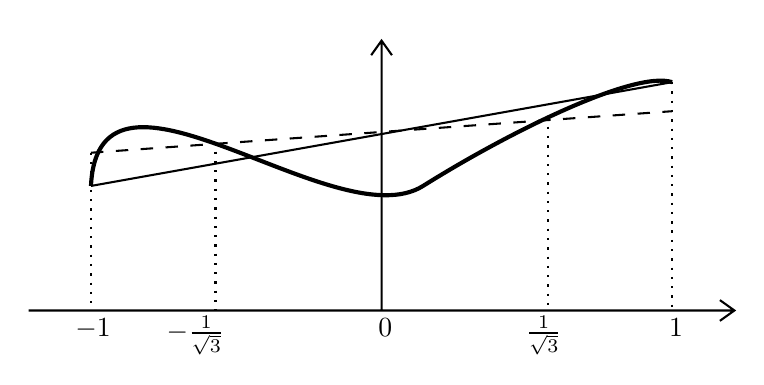
\begin{tikzpicture}[x=0.75pt,y=0.75pt,yscale=-1,xscale=1]
	%uncomment if require: \path (0,209); %set diagram left start at 0, and has height of 209

	%Shape: Axis 2D [id:dp7432814371793792]
	\draw  (130,140) -- (470,140)(300,10) -- (300,140) (463,135) -- (470,140) -- (463,145) (295,17) -- (300,10) -- (305,17)  ;
	%Straight Lines [id:da012820933470506057]
	\draw [color={rgb, 255:red, 0; green, 0; blue, 0 }  ,draw opacity=1 ][line width=0.75]  [dash pattern={on 0.84pt off 2.51pt}]  (160,64) -- (160,140) ;
	%Straight Lines [id:da052091442212324646]
	\draw [color={rgb, 255:red, 0; green, 0; blue, 0 }  ,draw opacity=1 ]   (160,80) -- (440,30) ;
	%Straight Lines [id:da9771507923640859]
	\draw [color={rgb, 255:red, 0; green, 0; blue, 0 }  ,draw opacity=1 ][line width=0.75]  [dash pattern={on 0.84pt off 2.51pt}]  (440,30) -- (440,140) ;
	%Straight Lines [id:da9708116128826352]
	\draw [color={rgb, 255:red, 0; green, 0; blue, 0 }  ,draw opacity=1 ][line width=0.75]  [dash pattern={on 0.84pt off 2.51pt}]  (380,47) -- (380,140) ;
	%Straight Lines [id:da13795556218359795]
	\draw [color={rgb, 255:red, 0; green, 0; blue, 0 }  ,draw opacity=1 ][line width=0.75]  [dash pattern={on 0.84pt off 2.51pt}]  (220,59) -- (220,140) ;
	%Straight Lines [id:da9729094667252978]
	\draw [color={rgb, 255:red, 0; green, 0; blue, 0 }  ,draw opacity=1 ] [dash pattern={on 4.5pt off 4.5pt}]  (160,64) -- (440,44) ;
	%Curve Lines [id:da34625381366262853]
	\draw [line width=1.5]    (160,80) .. controls (163.5,4.75) and (278,106.33) .. (320,80) .. controls (362,53.67) and (422,24.25) .. (440,30) ;

	% Text Node
	\draw (195,141.4) node [anchor=north west][inner sep=0.75pt]    {$-\frac{1}{\sqrt{3}}$};
	% Text Node
	\draw (368,141.4) node [anchor=north west][inner sep=0.75pt]    {$\frac{1}{\sqrt{3}}$};
	% Text Node
	\draw (437,142.4) node [anchor=north west][inner sep=0.75pt]    {$1$};
	% Text Node
	\draw (151,142.4) node [anchor=north west][inner sep=0.75pt]    {$-1$};
	% Text Node
	\draw (297,142.4) node [anchor=north west][inner sep=0.75pt]    {$0$};


	\end{tikzpicture}
	\caption{La linea spessa denota la $f( x)$, la linea sottile continua denota l'approssimazione che si ottiene con la formula del trapezio, mentre la linea sottile tratteggiata denota l'approssimazione con Gauss-Legendre.}
\end{figure}

La formula del trapezio integra in modo esatto fino a polinomi di grado $1$, mentre la \textbf{formula di Gauss-Legendre} integra in modo esatto fino a grado $3$.
\begin{align*}
I^{\text{GL}}_{1}( f) & =\sum\limits ^{2}_{i=0} \alpha _{i} f( x_{i}) =1\cdot f\left( -\frac{1}{\sqrt{3}}\right) +1\cdot f\left(\frac{1}{\sqrt{3}}\right)\\
I^{\text{trap}}_{1}( f) & =( b-a)\left[\frac{f( a) +f( b)}{2}\right] =f( -1) +f( 1)
\end{align*}

\subsection{Formule di Gauss-Legendre composite}
In modo simile a quanto fatto per le formule di Newton-Cotes, dividiamo l'intervallo $[a,b]$ in più sottointervalli, in ciascuno dei quali usiamo la formula di GL.

In questo caso, poiché GL non è una formula chiusa, in generale i polinomi interpolanti non si incontrano con continuità.

\begin{figure}[ht]
    \centering
% Pattern Info
\tikzset{
pattern size/.store in=\mcSize, 
pattern size = 5pt,
pattern thickness/.store in=\mcThickness, 
pattern thickness = 0.3pt,
pattern radius/.store in=\mcRadius, 
pattern radius = 1pt}
\makeatletter
\pgfutil@ifundefined{pgf@pattern@name@_yhmk61g9k}{
\pgfdeclarepatternformonly[\mcThickness,\mcSize]{_yhmk61g9k}
{\pgfqpoint{0pt}{-\mcThickness}}
{\pgfpoint{\mcSize}{\mcSize}}
{\pgfpoint{\mcSize}{\mcSize}}
{
\pgfsetcolor{\tikz@pattern@color}
\pgfsetlinewidth{\mcThickness}
\pgfpathmoveto{\pgfqpoint{0pt}{\mcSize}}
\pgfpathlineto{\pgfpoint{\mcSize+\mcThickness}{-\mcThickness}}
\pgfusepath{stroke}
}}
\makeatother

% Pattern Info
 
\tikzset{
pattern size/.store in=\mcSize, 
pattern size = 5pt,
pattern thickness/.store in=\mcThickness, 
pattern thickness = 0.3pt,
pattern radius/.store in=\mcRadius, 
pattern radius = 1pt}
\makeatletter
\pgfutil@ifundefined{pgf@pattern@name@_gfzj7aomp}{
\pgfdeclarepatternformonly[\mcThickness,\mcSize]{_gfzj7aomp}
{\pgfqpoint{0pt}{-\mcThickness}}
{\pgfpoint{\mcSize}{\mcSize}}
{\pgfpoint{\mcSize}{\mcSize}}
{
\pgfsetcolor{\tikz@pattern@color}
\pgfsetlinewidth{\mcThickness}
\pgfpathmoveto{\pgfqpoint{0pt}{\mcSize}}
\pgfpathlineto{\pgfpoint{\mcSize+\mcThickness}{-\mcThickness}}
\pgfusepath{stroke}
}}
\makeatother
\tikzset{every picture/.style={line width=0.75pt}} %set default line width to 0.75pt        

\begin{tikzpicture}[x=0.75pt,y=0.75pt,yscale=-1,xscale=1]
%uncomment if require: \path (0,240); %set diagram left start at 0, and has height of 240

%Shape: Polygon [id:ds6767593056546697] 
\draw  [pattern=_yhmk61g9k,pattern size=6pt,pattern thickness=0.75pt,pattern radius=0pt, pattern color={rgb, 255:red, 155; green, 155; blue, 155}] (313.67,185.6) -- (233.08,185.6) -- (231.35,70.48) -- (313.87,109.6) -- cycle ;
%Shape: Axis 2D [id:dp792326899605013] 
\draw  (109.44,185.72) -- (509.06,185.72)(136.83,30.69) -- (136.83,202.58) (502.06,180.72) -- (509.06,185.72) -- (502.06,190.72) (131.83,37.69) -- (136.83,30.69) -- (141.83,37.69)  ;
%Curve Lines [id:da6426647998245478] 
\draw [line width=1.5]    (193,117.11) .. controls (210.45,88.98) and (228.03,78.99) .. (245.08,78.67) .. controls (294.72,77.74) and (339.79,158.84) .. (363.35,112.94) .. controls (394.99,51.28) and (446.07,117.69) .. (513.82,76.38) ;
%Straight Lines [id:da06593695826492318] 
\draw  [dash pattern={on 4.5pt off 4.5pt}]  (250.27,80.67) -- (250.27,187.48) ;
%Straight Lines [id:da19011680567983746] 
\draw  [dash pattern={on 4.5pt off 4.5pt}]  (296.99,102.67) -- (296.99,185.48) ;
%Straight Lines [id:da14727304728561008] 
\draw  [dash pattern={on 4.5pt off 4.5pt}]  (333.33,123.48) -- (333.33,185.48) ;
%Straight Lines [id:da04415130495999009] 
\draw  [dash pattern={on 4.5pt off 4.5pt}]  (374.85,98.48) -- (374.85,186.48) ;
%Shape: Polygon [id:ds6999911861419973] 
\draw  [pattern=_gfzj7aomp,pattern size=6pt,pattern thickness=0.75pt,pattern radius=0pt, pattern color={rgb, 255:red, 155; green, 155; blue, 155}] (395.21,185.6) -- (313.67,185.6) -- (313.67,135.58) -- (395.72,85.48) -- cycle ;

% Text Node
\draw (212.89,195.26) node [anchor=north west][inner sep=0.75pt]    {$x_{k-1}$};
% Text Node
\draw (307.14,194.88) node [anchor=north west][inner sep=0.75pt]    {$x_{k}$};
% Text Node
\draw (397.21,197) node [anchor=north west][inner sep=0.75pt]    {$x_{k+1}$};
% Text Node
\draw (265,212.4) node [anchor=north west][inner sep=0.75pt]    {$I_{k}$};
% Text Node
\draw (342,214.4) node [anchor=north west][inner sep=0.75pt]    {$I_{k+1}$};
% Text Node
\draw (247.89,188.4) node [anchor=north west][inner sep=0.75pt]  [font=\scriptsize]  {$x_{1}^{\text G,k}$};
% Text Node
\draw (280.89,188.4) node [anchor=north west][inner sep=0.75pt]  [font=\scriptsize]  {$x_{2}^{\text G,k}$};
% Text Node
\draw (328.89,187.4) node [anchor=north west][inner sep=0.75pt]  [font=\scriptsize]  {$x_{1}^{\text G,k+1}$};
% Text Node
\draw (361.44,189) node [anchor=north west][inner sep=0.75pt]  [font=\scriptsize]  {$x_{2}^{\text G,k+1}$};
\end{tikzpicture}
\end{figure}

\begin{theorem}
    [Errore della formula di Gauss-Legendre composito a 2 nodi]
    Data $f\in C^4([a,b])$, esiste $\rho\in[a,b]$ tale che 
    \[
    E_\text{G2}^C(f)=\frac{H^4}{4320} (b-a)f^{(4)}(\rho)
    \]
\end{theorem}
Il grado di esattezza è $3$ e l'ordine di accuratezza è $4$.

\subsection{Polinomi di Legendre}
Cerchiamo un modo più semplice per trovare i nodi e pesi di GL\footnote{In realtà tali valori si trovano già tabulati in software di calcolo, per cui in genere non è necessario calcolarli.}.

Cominciamo introducendo la nozione di \textbf{polinomi ortogonali}\index{polinomio!ortogonale} rispetto a un peso, ovvero una funzione non negativa, integrabile e continua.
\begin{definition}
    Dato un insieme di polinomi $\mathcal P=\{p_k\}_{k=0}^n$, i suoi elementi sono detti \textbf{polinomi ortogonali} sull'intervallo $[a,b]$ rispetto al peso $w$ se
    \[
    \int_{a}^b p_k(x) p_m(x)w(x)\,dx=0\quad\forall k\ne x
    \]
\end{definition}

In particolare, se $w(x)\equiv 1$ e $[a,b]=[-1,1]$, i polinomi $L_k\in \mathcal P$ e tali che $L_k\in \mathbb P^k\ \forall k$ sono detti \textbf{polinomi di Legendre}\index{polinomio!di Legendre}.

Vale che
\[
\int_{-1}^{1} L_k(x) L_m(x) \, dx = \left(k + \frac{1}{2} \right)^{-1} \delta_{km},\quad \text{dove } \ \delta_{km}=\begin{cases}
    1&\text{se }k=m\\
    0&\text{se }k\ne m
\end{cases}
\]
Inoltre si può dimostrare che $\{L_k\}_{k=1}^n$ è una base per lo spazio dei polinomi di grado $n$ su $I$:
\begin{equation*}
\mathbb{P}^{n}(I) =\operatorname{span}\{L_{0}(x) ,L_{1}(x) ,\dotsc ,L_{n}(x)\} .
\end{equation*}
Presentiamo una formula ricorsiva per il calcolo dei polinomi di Legendre:
\begin{equation*}
\begin{cases}
L_{0}(x) =1\\
L_{1}(x) =x\\
L_{k+1} =\frac{2k+1}{k+1} xL_{k}(x) -\frac{k}{k+1} L_{k-1}(x) \quad \text{con} \quad k=1,2,\dots
\end{cases}
\end{equation*}

I polinomi di Legendre non sono l'unica famiglia di polinomi ortogonali: se ad esempio $w(x)=\frac{1}{\sqrt{1-x^2}}$, otteniamo i cosiddetti \textbf{polinomi di Chebyshev}\index{polinomio!di Chebyshev}.

\subsection{Approssimazione di integrali pesati}
Oltre a trovare i valori di pesi e nodi di GL, i polinomi di Legendre danno origine a una \textbf{formula di quadratura per integrali pesati}.

Approssimiamo l'integrale $I_w(f)$ in questo modo:
\[
I_w(f)=\int_{-1}^1f(x)w(x)\,dx\approx \sum_{i=0}^n f(x_i)\underbrace{\int_{-1}^1\varphi_i(x) w(x)\,dx}_{\alpha_i}=\sum _{i=0}^nf(x_i)\alpha_i,
\]
Dove gli $x_i$ sono gli zeri del polinomio di Legendre di grado $n+1$.

Il grado di esattezza della formula è $2n+1$, che si può dimostrare essere il massimo raggiungibile.

In particolare, se $w(x)\equiv 1$, troviamo i nodi di Gauss-Legendre ed i relativi pesi:
\begin{equation}
x_{i} = \text{zeri di} \ L_{n+1}(x) ,\quad \alpha _{i} =\frac{2}{( 1-x_{i})^{2}[ L_{n+1} '( x_{i})]^{2}} ,\quad i=0,\dotsc ,n.
\label{eq:nodi-gl}
\end{equation}


\subsection{Nodi e pesi di Gauss-Legendre-Lobatto (GLL)}
Come per i Gauss-Legendre, scegliamo strategicamente i nodi di quadratura, ma questa volta vogliamo che siano inclusi anche gli estremi.

Per $n\geqslant 0$, i \textbf{nodi di Gauss-Legendre-Lobatto}\index{nodi!di Gauss-Legendre-Lobatto} ed i relativi pesi sono dati da:
\begin{gather}
\begin{split}
x_{0} =-1,\quad &\left\{x_{i} \ \text{zeri di} \ L_{n} '(x) ,\quad i=1,\dotsc ,n-1\right\} ,\quad x_{n} =1,\\
&\alpha _{i} =\frac{2}{n( n+1)}\frac{1}{[ L_{n}( x_{i})]^{2}} ,\quad i=0,\dotsc ,n.
\end{split}
\label{eq:nodi-gll}
\end{gather}

Il grado di esattezza della formula è $2n-1$: due in meno di GL, poiché la scelta di due nodi (gli estremi) non è strategica.

\textbf{NB.}
Sull'intervallo generico $[ a,b]$ i nodi di GL e GLL si ottengono da \eqref{eq:nodi-gl} e da \eqref{eq:nodi-gll} con la stessa trasformazione lineare vista nella sezione \ref{sec:interpolazione-non-equispaziata} per l'interpolazione non equispaziata, mentre per i pesi si usa un'altra trasformazione:
\begin{equation*}
\hat{x}_{i} =\frac{a+b}{2} +\frac{b-a}{2} x_{i}, \quad \hat \alpha_i=\frac{b-a}{2}\alpha_i,\quad i=0,\dotsc ,n.
\end{equation*}

\subsection{Errore delle formule di GL e GLL}
\index{errore!di Gauss-Legendre}
\index{errore!di Gauss-Legendre-Lobatto}
Data $f$ sufficientemente regolare, vale la seguente rappresentazione dell'errore:
\begin{equation*}
| E_{n}(f)| \leqslant \frac{C}{n^{5}}\Vert f\Vert _{s}
\end{equation*}
dove
\begin{equation*}
\Vert f\Vert _{s} =\left(\sum\limits ^{s}_{k=0}\left\Vert f^{(k)}\right\Vert ^{2}_{L^{2}( -1,1)}\right)^{1/2}
\end{equation*}
nel quale
\begin{equation*}
\Vert f\Vert _{L^{2}( -1,1)} =\left[\int\nolimits ^{1}_{-1}[ f(x)]^{2} \dx\right]^{1/2} .
\end{equation*}

Per concludere il capitolo, presentiamo nella tabella \ref{tab:gradi-ordini} un riassunto dei principali risultati di accuratezza ed esattezza delle formule viste.

\begin{table}[ht]
\centering
{\renewcommand{\arraystretch}{1.3}% for the vertical padding
\begin{tabular}{lcc}
\toprule
   & grado di esattezza & ordine di accuratezza \\
\midrule
 Punto medio semplice & $1$ &  \\
 Trapezio semplice & $1$ &  \\
 CS semplice & $3$ &  \\
 $n$ pari & $n+1$ &  \\
 $n$ dispari & $n$ &  \\
\hline
 Punto medio composito & $1$ & $2$ \\
 Trapezio composito & $1$ & $2$ \\
 CS composito & $3$ & $4$ \\
\hline
 NC, $n$ pari & $n+1$ & $n+3$ \\
 NC, $n$ dispari & $n$ & $n+2$ \\
 NC composite, $n$ pari & $n+1$ & $n+2$ \\
 NC composite, $n$ dispari & $n$ & $n+1$ \\
\hline
 GL & $2n+1$ &  \\
 GLL & $2n-1$ &  \\
 \bottomrule
\end{tabular}
}
\caption{Tabella riassuntiva dei gradi di esattezza e ordini di accuratezza dei metodi numerici analizzati.}
\label{tab:gradi-ordini}
\end{table}
